\subsection*{Inhalt}
\begin{itemize}
	\item Abzählmethoden
	\item Rekursionen
	\item geordnete Mengen, Scheduling
	\item Anwendungen der linearen Algebra, z.B. Information Retrieval
\end{itemize}

\section{Abzählmethoden}

\subsection[Kardinalität paarweise disjunkter Mengen und des karthesischen Produkts]{} 
\label{subsec:disjcup(a)+kard(b)}
$S_1, \dots, S_n$ endliche Mengen
\begin{enumerate}
	\item  Sind $S_1, \dots, S_n$ paarweise disjunkt, so 
	\[\abs{S_1 \cup \dots \cup S_n} = \sum_{i=1}^{n}\abs{S_i}\]
	\item 
	\footnote{$S_1 \times \dots \times S_n = \aset{(s_1, \dots, s_n) : s_i \in S_i}$; Ist  $s_1 = s_2 = \dots = s_n = s  $ so $\underset{\leftarrow n \rightarrow}{s \times \dots \times s =: S^n}$}
	\[ \abs{S_1 \times \dots \times S_n} = \prod_{i=1}^n \abs{S_i} 
	 \]
\end{enumerate}

\subsection[Beispiel : Kardinalität der Vereinigung paarweise disjunkter Mengen]{Beispiele}

\begin{enumerate}
	\item
	Es gibt $2^n$ Wörter der Länge $n$ über $\aset{0,1}$
	\\ Allgemein Alphabet $S$ der Größe $q$, so gibt es $q^n$ Wörter der Länge $n$ über $S$
	
	\item[c)] Wie viele 3-stellige Zahlen (im Dezimalsystem; ggf. mit führenden Nullen) gibt es, die mindestens eine $1$ enthalten?
	Dafür gibt es mehrere\textbf{} Möglichkeiten:
	\begin{enumerate} %TODO Zahlen  + Mögl.
		\item $S =$ Menge aller 3.st. Zahlen mit mindestens einer 1.
		
		$S_1 = \aset{s \in S : \text{ an erster Stelle von } s \text{ steht } 1}$
		\\$S_2 = \aset{s \in S : \text{ die erste 1 von } s \text{ steht an 2. Stelle}}$
		\\$S_3 = \aset{s \in S : \text{ die erste 1 von } s \text{ steht an 3. Stelle}}$
		
		$S = S_1\: \dot{\cup}\; S_2 \;\dot{\cup}\; S_3$ 
		
		$S_1 = \aset{1} \times \aset{0, \dots, 9} \stackrel{\ref{subsec:disjcup(a)+kard(b)}b}{\Rightarrow} 
		\abs{S_1} = 1 \cdot 10 \cdot 10 = 100$
		\\
		$S_2 = \aset{0, 2, \dots, 9} \times \aset{1} \times \aset{0, \dots, 9} 
		\stackrel{\ref{subsec:disjcup(a)+kard(b)}b}{\Rightarrow} 
		\abs{S_2} = 9\cdot 1 \cdot 10 = 90$
		\\
		$S_3 = \aset{0, 2 \dots, 9} \times \aset{0, 2, \dots, 9} \times \aset{1}
		\stackrel{\ref{subsec:disjcup(a)+kard(b)}b}{\Rightarrow} 
		\abs{S_3} = 9 \cdot 9 \cdot 1 = 81$
		
		\ref{subsec:disjcup(a)+kard(b)}a: \quad 
		$\abs{S} = \abs{S_1} + \abs{S_2} + \abs{S_3} = 271$
		
		\item 
		$T_i = \aset{s \in S : s \text{ enthält mindestens } i \text{ mal die 1}}, i = 1, 2, 3, S = T_1 \;\dot{\cup}\; T_2 \;\dot{\cup}\; T_3$ 
		
		\begin{itemize}		
		
		\item $T_1 = T_1^1 \;\dot{\cup}\; T_1^2 \;\dot{\cup}\; T_1^3$,
	    \; $T_i^j = \aset{s \in T_1 : 1 \text{ steht an Stelle } j}$
	   
	    $\abs{T_1^1} = \abs{T_1^2} = \abs{T_1^3} = 9 \cdot 9 \cdot 1 = 81, 
	    \quad \abs{T_1} = 3 \cdot 81 = 243$ (\ref{subsec:disjcup(a)+kard(b)}) 
	    
	    \item  $T_2 = T_2^1 \cup T_2^2 \cup T_2^3$, 
	    \; $T_2^j = \aset{s \in T_2 : \text{ an der Stelle } j \text{ steht keine 1}}$
	    
	    $\abs{T_2^1} = \abs{T_2^2} = \abs{T_2^3} = 9$
	    \quad $ \abs{T_2} = 3 \cdot 9 = 27$
	    
	   \item  $\abs{T_3} = 1$
	    
	    \end{itemize}
	    
	    $\abs{S} = \abs{T_1 } + \abs{T_2} + \abs{T_3} = 271$
	    
	    \item
	    $G = \aset{0, \dots, 9}^3, \abs{G} = 1000$
	    
	    $S = G \without{\underbrace{x \in G : x \text{ enthält keine 1}}_{\aset{0, 2, \dots 9}^3}}$
	    
	    $\abs{\aset{0, 2, \dots, 9}^3} \stackrel{\ref{subsec:disjcup(a)+kard(b)}b}{=} 
	    9 \cdot 9 \cdot 9 = 729$
	    
	    $\abs{S} = 1000 - 729 = 271$
	 		
	\end{enumerate}
	
\end{enumerate}

\subsection*{Techniken im Beispiel}
\begin{itemize}
	\item Zerlegen einer abzählbaren Menge in disjunkte Teilmengen
	\item Abzählen des Komplements
\end{itemize}

Wie lässt sich \ref{subsec:disjcup(a)+kard(b)}a 
verallgemeinern, falls die $S_i$ nicht notwendig disjunkt?

$n=2$ : 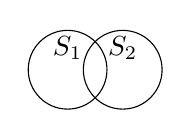
\begin{tikzpicture}
	\draw (0,0) circle (.5cm) node[above]{$S_1$};
	\draw (.7,0) circle (.5cm) node[above]{$S_2$};	
\end{tikzpicture}
$\abs{S_1 \cup S_2} = \abs{S_1} + \abs{S_2} - \abs{S_1 \cap S_2}$

$n=3$ : 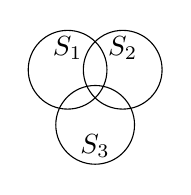
\begin{tikzpicture}
	\draw (0,0) circle (.5cm) node[above]{$S_1$};
	\draw (.7,0) circle (.5cm) node[above]{$S_2$};
	\draw (.35,-0.7) circle (.5cm) node[below]{$S_3$};	
\end{tikzpicture}
$\abs{S_1 \cup S_2 \cup S_3} = \abs{S_1} + \abs{S_2} + \abs{S_3}
                             - \abs{S_1 \cap S_2} - \abs{S_1 \cap S_3} - \abs{S_2 \cap S_3}
                             + \abs{S_1 \cap S_2 \cap S_3}$
                             
Allgemein gilt:

\subsection{Einschließungs-Ausschließungsprinzip}
\label{subsec:einausschliessprinzip}

\[\abs{ S_1 \cup \dots \cup S_n} = \sum_{k=1}^n(-1)^{k+1} \sum_{1 \leq i_1 < i_2 < \dots < i_k \leq n}{\abs{S_{i_i} \cap \dots \cap S_{i_k}}} \]
(Beweis WHK, 2.32)

\subsection{Beispiel : Einschließungs-Ausschließungsprinzip}

\begin{enumerate}
	\item Wie viele 8-stellige Zahlen (Dezimalsystem, mit führenden Nullen) enthalten nicht alle ungerade Ziffern?
	
	$S =$ Menge aller 8-st. Zahlen.
	\\$S_i = \aset{s \in S : s \text{ enthält nicht } i}, i = 1, 3, 5, 7, 9 $
	
	$\abs{S_1 \cup S_3 \cup S_5 \cup S_7 \cup S_9}$
	
	\ref{subsec:einausschliessprinzip} anwenden 
	($n=5 $)
	
	\begin{tabular}{l@{ : }lllc}

	$k=1$ 
	& $\underset{=9^8}{\abs{S_1}}, \dots, \underset{=9^8}{\abs{S_9}}$
	&
	& $5 \cdot 9^8$ 
	& (+)\\
	
	
	$k=2$ 
	& $\underbrace{\abs{S_1 \cap S_3}}_{\text{8-st. ohne 1, ohne 3}} = 8^8$, entsprechend $\abs{S_1 \cup S_5}, \dots \abs{S_7 \cap S_9}$ 
	& 10 mal 
	& $10 \cdot 8^8$ 
	&(-) \\
	
	$k=3$ 
	& $\abs{S_1 \cap S_3 \cap S_5} = 7^8$ 
	& 10 mal 
	&$10 \cdot 7^8$ 
	&(+) \\
	
 	$k=4$
 	& $\abs{S_1 \cap S_3 \cap S_5 \cap S_7} = 6^8$ 
 	& 5 mal 
 	& $5 \cdot 6^8$ 
 	& (-) \\
 	
 	$k=5$ 
 	& $\abs{S_1 \cap S_3 \cap S_5 \cap S_7 \cap S_9} = 5^8$ 
 	& 1 mal 
 	& $5^8$ 
 	& (+) \\
	 \end{tabular}
 		
	
	$\abs{S_1 \cup S_3 \cup S_5 \cup S_7 \cup S_9} = 5 \cdot 9^8 - 10 \cdot 8^8 + 10\cdot 7^8 - 5 \cdot 6^8 + 5^8 = 97102000$
\end{enumerate}
                             


















